\documentclass{article}
\usepackage[utf8]{inputenc}
\usepackage{amsmath, amssymb}
\usepackage[linesnumbered,ruled,vlined]{algorithm2e}
\usepackage{tikz}
\usetikzlibrary{shapes.geometric, arrows, positioning, fit}
\usepackage{geometry}
\geometry{a4paper, margin=1in}

\title{\textbf{Adaptive HNSW Search via Entry-Point Topology and Aggregate Recall Curves}}
\author{Algorithm \& Logic Specification}
\date{}

\begin{document}

\maketitle

\section{Introduction}
In Hierarchical Navigable Small World (HNSW) graphs, the \texttt{ef} (exploration factor) parameter strictly controls the trade-off between search speed and recall. A constant \texttt{ef} across all queries is computationally inefficient due to the vast variance in query difficulty. The \textbf{2Metric Adaptive EF} architecture solves this by extracting structural signals from an initial low-cost graph probe. These signals are mapped to a calibrated \textit{Aggregate Recall Curve} table, assigning the optimal \texttt{ef} dynamically on a per-query basis.

\section{The Dual-Metric Estimator}
The estimator isolates the two primary causes of search failure in HNSW: global routing errors (upper layers) and local hub entrapment (base layer).

\subsection{Drop-off Entry Point Distance ($d_{ep}$) -- Global Routing Signal}
The $d_{ep}$ metric measures the absolute distance from the query to the final node of the upper-layer greedy descent (the exact point where the search drops into Layer 0).
\begin{equation}
    d_{ep} = \text{dist}(q, \text{Layer}_0 \text{ Entry Node})
\end{equation}
\begin{itemize}
    \item \textbf{High $d_{ep}$:} The upper layers were sparse and routed poorly, dropping the search far away from the true nearest neighbors. Layer 0 will require a massive exhaustive crawl to recover. Hard query.
    \item \textbf{Low $d_{ep}$:} The upper layers successfully dropped the search precisely in the target neighborhood. Easy query.
\end{itemize}

\subsection{Topological Rank Entrapment ($RV$) -- Local Topological Signal}
$RV$ measures the degree to which the Layer-0 search wastes iterations revisiting identical hub nodes, weighted heavily toward early encounters via exponential decay ($\gamma$).
\begin{equation}
    RV = \frac{\sum_{i=1}^N \mathbf{I}(e_i \text{ is revisit}) \cdot e^{-\gamma \cdot (i/N)}}{\sum_{i=1}^N e^{-\gamma \cdot (i/N)}}
\end{equation}
\begin{itemize}
    \item \textbf{High $RV$:} The local neighborhood is entangled with massive hubs. Hard query.
    \item \textbf{Low $RV$:} The graph structure leads linearly to the target. Easy query.
\end{itemize}

\section{Algorithms and Pseudocode}

\subsection{Phase 1: The Probe Phase}
\begin{algorithm}[H]
\DontPrintSemicolon
\SetAlgoLined
\KwIn{HNSW Graph $G$, Query $q$, Probe Cap $C$, Decay $\gamma$}
\KwOut{Estimated Signals $(d_{ep}, RV)$}

$ep \leftarrow \text{GreedyDescent}(G_{upper}, q)$ \tcp*{Drop to Layer 0}
$d_{ep} \leftarrow \text{dist}(q, ep)$\;
$visited \leftarrow \{ep\}$, $candidates \leftarrow \{ep\}$, $edges \leftarrow []$\;

\While{$candidates \neq \emptyset$ \textbf{and} $|evaluated| \leq C$}{
    $curr \leftarrow candidates.pop\_closest()$\;
    \For{$nbr \in \text{neighbors}(curr)$}{
        $d \leftarrow \text{dist}(q, nbr)$\;
        $is\_revisit \leftarrow nbr \in visited$\;
        $edges.append( (d, is\_revisit) )$\;
        \If{\textbf{not} $is\_revisit$}{
            $visited.insert(nbr)$; $candidates.push(nbr)$\;
        }
    }
}
Sort $edges$ by $d$ ascending\;
$W_{tot} \leftarrow 0$, $W_{vis} \leftarrow 0$, $N \leftarrow length(edges)$\;
\For{$i \leftarrow 1$ \KwTo $N$}{
    $w \leftarrow \exp(-\gamma \cdot (i / N))$\;
    $W_{tot} \leftarrow W_{tot} + w$\;
    \If{$edges[i].is\_revisit$}{ $W_{vis} \leftarrow W_{vis} + w$\; }
}
$RV \leftarrow W_{vis} / \max(W_{tot}, \epsilon)$\;
\Return $(d_{ep}, RV)$
\caption{HNSW Dual-Metric Probe Extraction}
\end{algorithm}

\vspace{1em}

\subsection{Phase 2: Table Calibration via Aggregate Recall Curves}
Rather than recording individual required EFs and suffering from high within-bin variance, the table generator groups training queries into a $32 \times 32$ grid of $(d_{ep}, RV)$ bins. It steps through $ef$ values using an \textbf{Inverse-Slope Dynamic Increment} until the \textit{aggregate average recall} of the entire bin satisfies the target recall constraint. 

To save computational overhead, an early-stopping $\epsilon$-threshold aborts evaluations for any query that flatlines mathematically.

\begin{algorithm}[H]
\DontPrintSemicolon
\SetAlgoLined
\KwIn{Query Stream $Q$, Graph $G$, Target Recall $T_R$, Min Step $k_{half}$}
\KwOut{2D Grid Mapping $(d_{ep}, RV) \rightarrow \text{Curve}(ef, avg\_recall)$}

\For{each bin $B \in Grid(d_{ep}, RV)$}{
    $ef_1 \leftarrow k$, $ef_2 \leftarrow k \times 1.5$\;
    $rec_1 \leftarrow \text{AvgRecall}(B, ef_1)$\;
    $rec_2 \leftarrow \text{AvgRecall}(B, ef_2)$\;
    $B.curve \leftarrow [(ef_1, rec_1), (ef_2, rec_2)]$\;
    
    $latest\_ef \leftarrow ef_2$, $prev\_ef \leftarrow ef_1$\;
    $latest\_rec \leftarrow rec_2$, $prev\_rec \leftarrow rec_1$\;
    $ef\_diff \leftarrow latest\_ef - prev\_ef$\;
    
    \While{$T_R - latest\_rec > 1e^{-4}$ \textbf{and} $latest\_ef < max\_ef$}{
        $recall\_diff \leftarrow latest\_rec - prev\_rec$\;
        \If{$recall\_diff < 1e^{-6}$}{
            \textbf{break}\; \tcp*{Epsilon Early Stopping (Plateau)}
        }
        \tcp{Proportional Guess using Inverse-Slope}
        $step \leftarrow \text{int}\left( ef\_diff \cdot \frac{T_R - latest\_rec}{recall\_diff} \right)$\;
        $ef\_diff \leftarrow \max(step, k_{half})$ \tcp*{Strict floor guard}
        
        $next\_ef \leftarrow \min(latest\_ef + ef\_diff, max\_ef)$\;
        $next\_rec \leftarrow \text{AvgRecall}(B, next\_ef)$\;
        $B.curve.push(next\_ef, next\_rec)$\;
        
        $prev\_ef \leftarrow latest\_ef$, $prev\_rec \leftarrow latest\_rec$\;
        $latest\_ef \leftarrow next\_ef$, $latest\_rec \leftarrow next\_rec$\;
    }
}
\caption{Dynamic Aggregate Curve Calibration}
\end{algorithm}

\vspace{1em}

\subsection{Phase 3: The Adaptive Search Loop with Query-Weighted Floor}
To prevent artificial inflation via cumulative feedback loops, the online search utilizes a \textbf{Static Query-Weighted Table Average} as a safe floor mechanism. The overall required $ef$ across all valid curves in the lookup table is averaged, ensuring easy queries never drop beneath the dataset's topological baseline.

\begin{algorithm}[H]
\DontPrintSemicolon
\SetAlgoLined
\KwIn{Query $q$, Graph $G$, Lookup Table $T$, Table Average Floor $EF_{avg}$}
\KwOut{Nearest Neighbors for $q$}

$(d_{ep}, RV) \leftarrow \text{ProbeExtraction}(G, q)$\;
$ef_{lookup} \leftarrow T\text{.find\_minimum\_ef\_for\_target\_recall}(d_{ep}, RV)$\;

\tcp{Floor isolated strictly to static map baseline}
$ef_{dyn} \leftarrow \max(ef_{lookup}, EF_{avg})$\;
$ef_{dyn} \leftarrow \max(ef_{dyn}, k)$\;

$G.setEf(ef_{dyn})$\;
$results \leftarrow G.searchKnn(q)$\;
\Return $results$
\caption{Online Adaptive EF Search Loop}
\end{algorithm}

\section{System Architecture Visualization}

\begin{center}
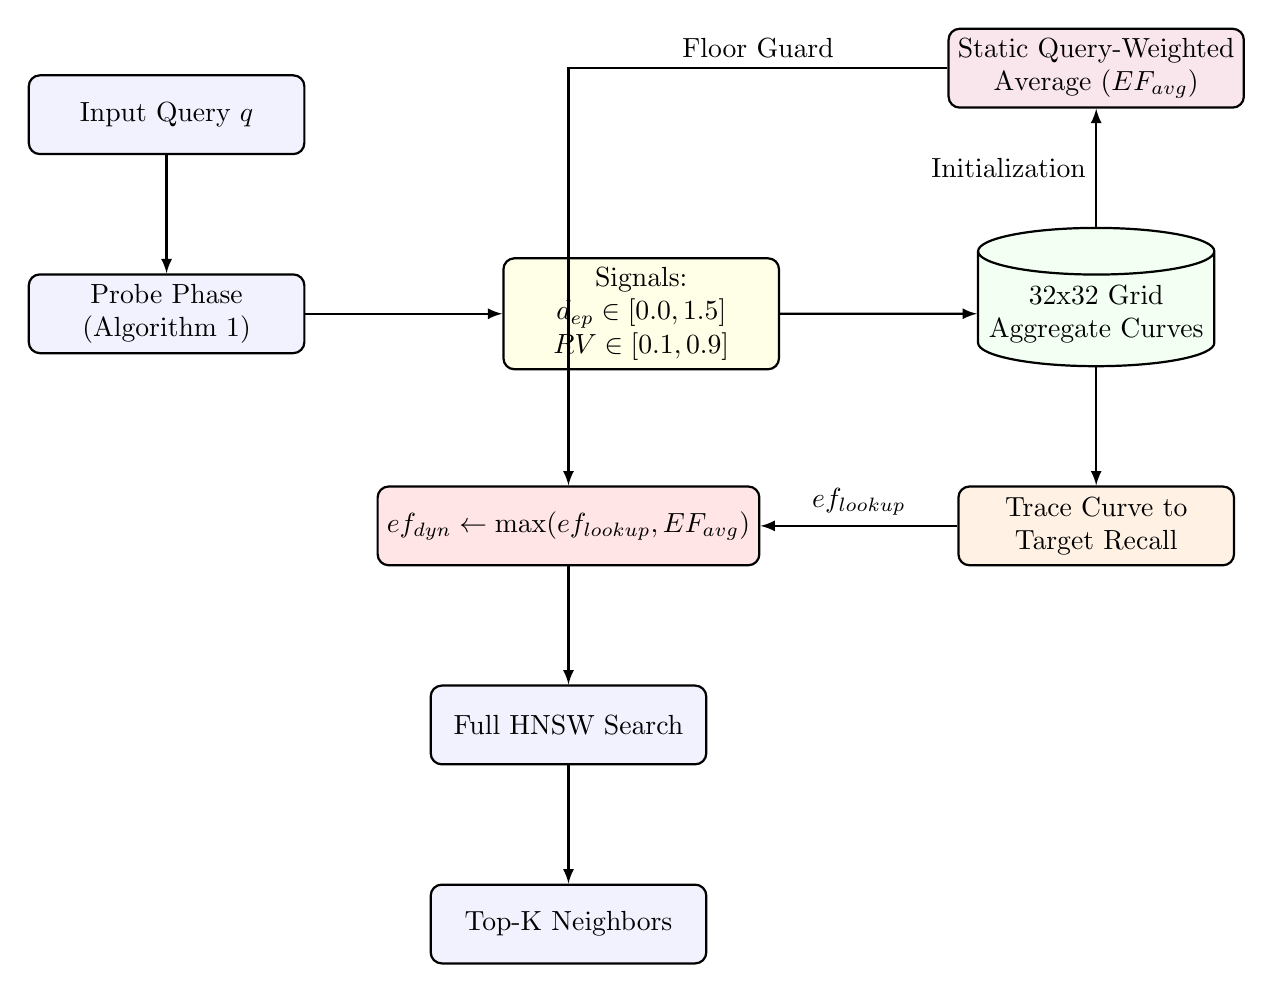
\begin{tikzpicture}[
    node distance=1.5cm and 2.5cm,
    box/.style={rectangle, draw, rounded corners, align=center, thick, fill=blue!5, minimum width=3.5cm, minimum height=1cm},
    data/.style={cylinder, draw, shape border rotate=90, aspect=0.2, align=center, thick, fill=green!5, minimum width=3cm, minimum height=1cm},
    arrow/.style={-latex, thick}
]

% Nodes
\node (query) [box] {Input Query $q$};
\node (probe) [box, below=of query] {Probe Phase\\(Algorithm 1)};
\node (signals) [box, right=of probe, fill=yellow!10] {Signals:\\$d_{ep} \in [0.0, 1.5]$\\$RV \in [0.1, 0.9]$};
\node (table) [data, right=of signals] {32x32 Grid\\Aggregate Curves};
\node (avg) [box, above=of table, fill=purple!10] {Static Query-Weighted\\Average ($EF_{avg}$)};
\node (lookup) [box, below=of table, fill=orange!10] {Trace Curve to\\Target Recall};
\node (ef) [box, left=of lookup, fill=red!10] {$ef_{dyn} \leftarrow \max(ef_{lookup}, EF_{avg})$};
\node (search) [box, below=of ef] {Full HNSW Search};
\node (result) [box, below=of search] {Top-K Neighbors};

% Arrows
\draw [arrow] (query) -- (probe);
\draw [arrow] (probe) -- (signals);
\draw [arrow] (signals) -- (table);
\draw [arrow] (table) -- (avg) node[midway, left] {Initialization};
\draw [arrow] (table) -- (lookup);
\draw [arrow] (lookup) -- (ef) node[midway, above] {$ef_{lookup}$};
\draw [arrow] (avg.west) -| (ef.north) node[pos=0.25, above] {Floor Guard};
\draw [arrow] (ef) -- (search);
\draw [arrow] (search) -- (result);

\end{tikzpicture}
\end{center}

\section{Conclusion}
By utilizing $d_{ep}$ (measuring structural routing failures) orthogonally against $RV$ (measuring local network entanglement), the 2Metric system successfully splits topological difficulty into its two physical causes. The resulting Aggregate Recall Curves smoothly interpolate required limits, while the Query-Weighted Floor safely halts runaway error spiraling, enabling near-perfect target recall achievement with significantly reduced average computation.

\end{document}
